% Simple 48in x 36in landscape poster template (beamerposter)
% Compile with: pdflatex poster.tex   (or `make` from this directory)
\documentclass[final]{beamer}
\usepackage[size=custom, width=121.92, height=91.44, scale=1.05]{beamerposter} % 48in x 36in in cm
\usepackage[utf8]{inputenc}
\usepackage{graphicx}
\usepackage{amsmath,amssymb}
\usepackage{booktabs}

% Figures live in the report directory
\graphicspath{{../report/figures/}}

% ---- Berkeley-accented theme: colored title bars, white block bodies ----
\definecolor{berkeleyblue}{HTML}{003262}
\definecolor{californiagold}{HTML}{FDB515}

\usetheme{default}
\setbeamertemplate{navigation symbols}{}
\setbeamercolor{block title}{fg=white, bg=berkeleyblue}
\setbeamercolor{block body}{fg=black, bg=white}
\setbeamercolor{background canvas}{bg=white}
\setbeamertemplate{itemize items}[circle]
\setbeamerfont{block title}{series=\bfseries}
\setbeamercolor{itemize item}{fg=berkeleyblue}
\setbeamercolor{itemize subitem}{fg=berkeleyblue}

\title{
Subject-Level Calibration Heterogeneity is Stable Across LLM Families and Scales: A Statistical Audit of MMLU}
\author{Jennifer Zhang, John Wright}
\institute{Department of Statistics, University of California, Berkeley}

\begin{document}
\begin{frame}[t]

\begin{block}{}
  \begin{columns}[c]
    \begin{column}{0.12\linewidth}
      \centering
      \IfFileExists{../report/figures/berkeley_logo.pdf}{%
        \includegraphics[width=0.85\linewidth]{berkeley_logo.pdf}%
      }{%
        \IfFileExists{../report/figures/berkeley_logo.png}{%
          \includegraphics[width=0.85\linewidth]{berkeley_logo.png}%
        }{}%
      }
    \end{column}
    \begin{column}{0.76\linewidth}
      \centering
      {\VeryHuge \inserttitle}\\[0.5em]
      {\Large \insertauthor}\\
      {\large \insertinstitute}
    \end{column}
    \begin{column}{0.12\linewidth}
    \end{column}
  \end{columns}
\end{block}

\begin{columns}[t]

  % ------------------------- Left column -------------------------
  \begin{column}{0.33\linewidth}

    \begin{block}{Motivation\vphantom{g}}
      \begin{itemize}
        \item A model is \textbf{well-calibrated} if its stated confidence
          matches its accuracy (e.g., 80\% confident $\Rightarrow$ correct
          80\% of the time).
        \item Calibration is usually reported as one aggregate scalar (ECE),
          hiding \emph{where} miscalibration concentrates:
      \end{itemize}
\[
  \mathrm{ECE} = \sum_b \frac{|B_b|}{n}\,|\mathrm{acc}(B_b) - \mathrm{conf}(B_b)|
\]
      \begin{itemize}
        \item \textbf{Questions:} where does miscalibration concentrate,
          and how much; is that pattern consistent across models; what
          drives it (question features, model scale)?
      \end{itemize}
    \end{block}

    \begin{block}{Data \& Methods}
      \begin{itemize}
        \item \textbf{Data:} MMLU --- 14{,}042 four-option questions, 57
          subjects, 4 domains; subject sizes 100--1{,}534 (median 173).
        \vspace{0.3em}
        \item \textbf{Confidence:} renormalized softmax over the four
          answer tokens:
\[
  c_i = \max_{a \in \{A,B,C,D\}} \frac{e^{\ell_a}}{\sum_{a'} e^{\ell_{a'}}}
\]
          {\small (bounded below at $0.25$ by construction --- four-way
          softmax.)}
        \item \textbf{Models:} GPT-4o-mini, Llama-3-8B-Instruct,
          Qwen-2.5-\{0.5B, 1.5B, 3B, 7B, 14B\}-Instruct. Outcome: signed
          \emph{calibration gap} $\mathrm{gap}_i = c_i - y_i$, $y_i \in
          \{0,1\}$ correctness (positive under overconfidence).
        \vspace{0.3em}
        \item \textbf{Model:} three-level mixed model (questions $\to$
          subjects $\to$ domains), fit via REML:
\[
  \mathrm{gap}_{ijk} = \mu + \mathbf{x}_{ijk}^\top\boldsymbol{\beta}
    + u_k + v_{jk} + \varepsilon_{ijk}
\]
          {\small $u_k$: domain random effect; $v_{jk}$: subject-within-domain
          random effect; $\varepsilon_{ijk}$: question-level residual.}
        \item \textbf{Per-subject test:} one-sample $t$-test on question-level
          gaps ($H_0$: mean gap $=0$), BH-FDR corrected across 57 subjects at
          $\alpha=0.05$ (detailed next column).
        \item \textbf{Cross-model stability:} Spearman correlation of
          subject-level ECE across all 15 pairs among the 6 larger models,
          with bootstrap 95\% CIs (detailed in Cross-Model Stability panel).
      \end{itemize}
    \end{block}

    \begin{block}{Variance Decomposition}
      \begin{itemize}
        \item Most calibration-gap variance is at the question level
          (92.0--98.5\%); domain variance collapses to zero.
        \item Between-subject ICC spans nearly $5\times$ across models ---
          small in absolute terms, but (next block) large enough to organize
          a $3.8$--$13.0\times$ range in subject-level miscalibration.
      \end{itemize}

      \vspace{0.5em}
      \begin{center}
      \small
      \begin{tabular}{lr}
        \toprule
        Model & ICC$_{\text{subject}}$ \\
        \midrule
        GPT-4o-mini            & 0.079 \\
        Llama-3-8B             & 0.020 \\
        Qwen-2.5-0.5B          & 0.018 \\
        Qwen-2.5-1.5B          & 0.017 \\
        Qwen-2.5-3B            & 0.051 \\
        Qwen-2.5-7B            & 0.049 \\
        Qwen-2.5-14B           & 0.059 \\
        \bottomrule
      \end{tabular}
      \end{center}
      {\small ICC$_{\text{subject}}$: share of total calibration-gap variance
      attributable to subject (domain variance is estimated at zero for all
      models).}
    \end{block}

    \begin{block}{Where Calibration Fails}
      \begin{itemize}
        \item \textbf{Every model is overconfident on average:} intercept
          ($\mu$) positive for all seven models, $0.18$--$0.31$ (Guo et al.\
          2017; Kadavath et al.\ 2022).
        \vspace{0.3em}
        \item \textbf{Worst, every model $>$1B:} \texttt{virology},
          \texttt{professional\_law} (top-10); college-STEM cluster ---
          \texttt{abstract\_algebra}, \texttt{college\_mathematics},
          \texttt{machine\_learning} (top-5, 4 of 6 models).
        \item \textbf{Best, every model:} \texttt{marketing},
          \texttt{high\_school\_psychology} (lowest ECE).
        \item \textbf{Pattern:} specialization level, not domain ---
          college subjects miscalibrate more than their high-school
          counterparts.
      \end{itemize}

      \vspace{0.3em}
      \begin{center}
        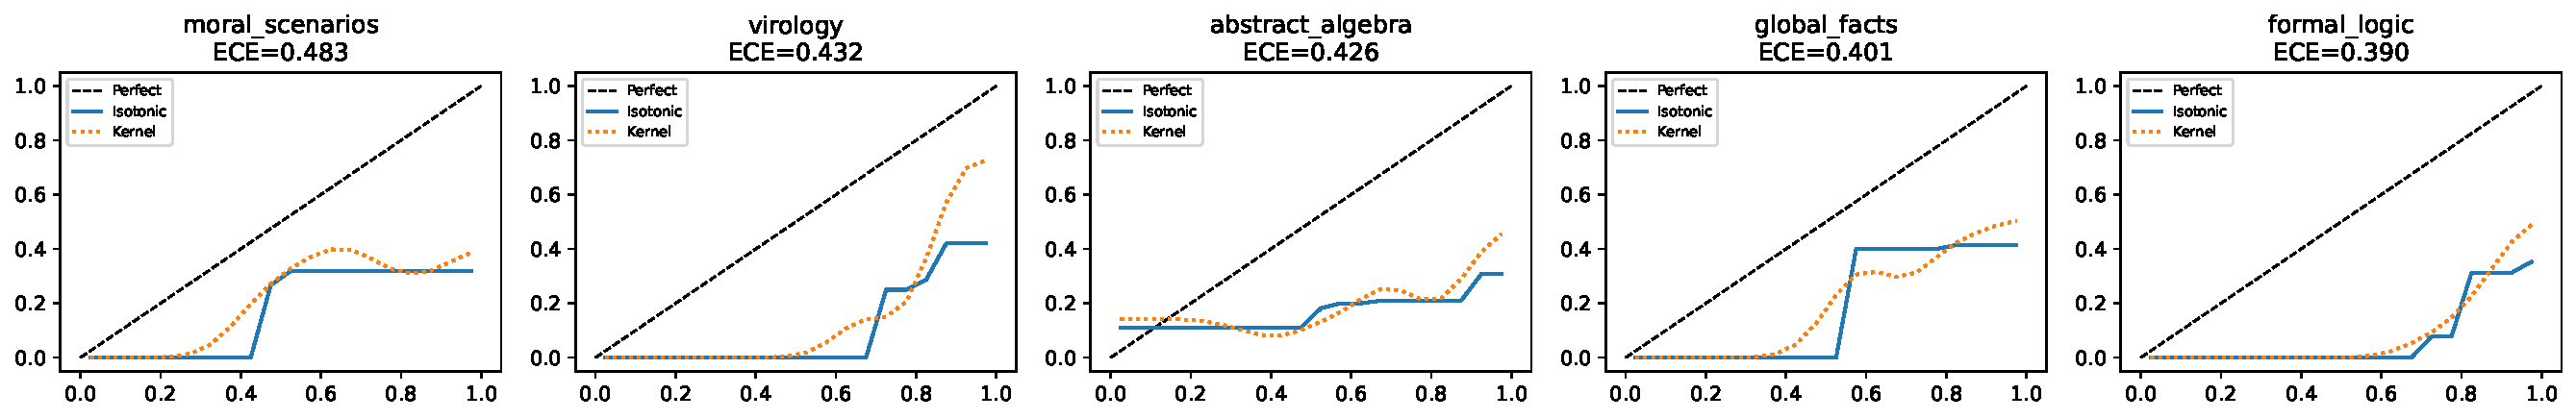
\includegraphics[width=0.95\linewidth]{top5_miscalibrated_gpt4o.pdf}\\[0.2em]
        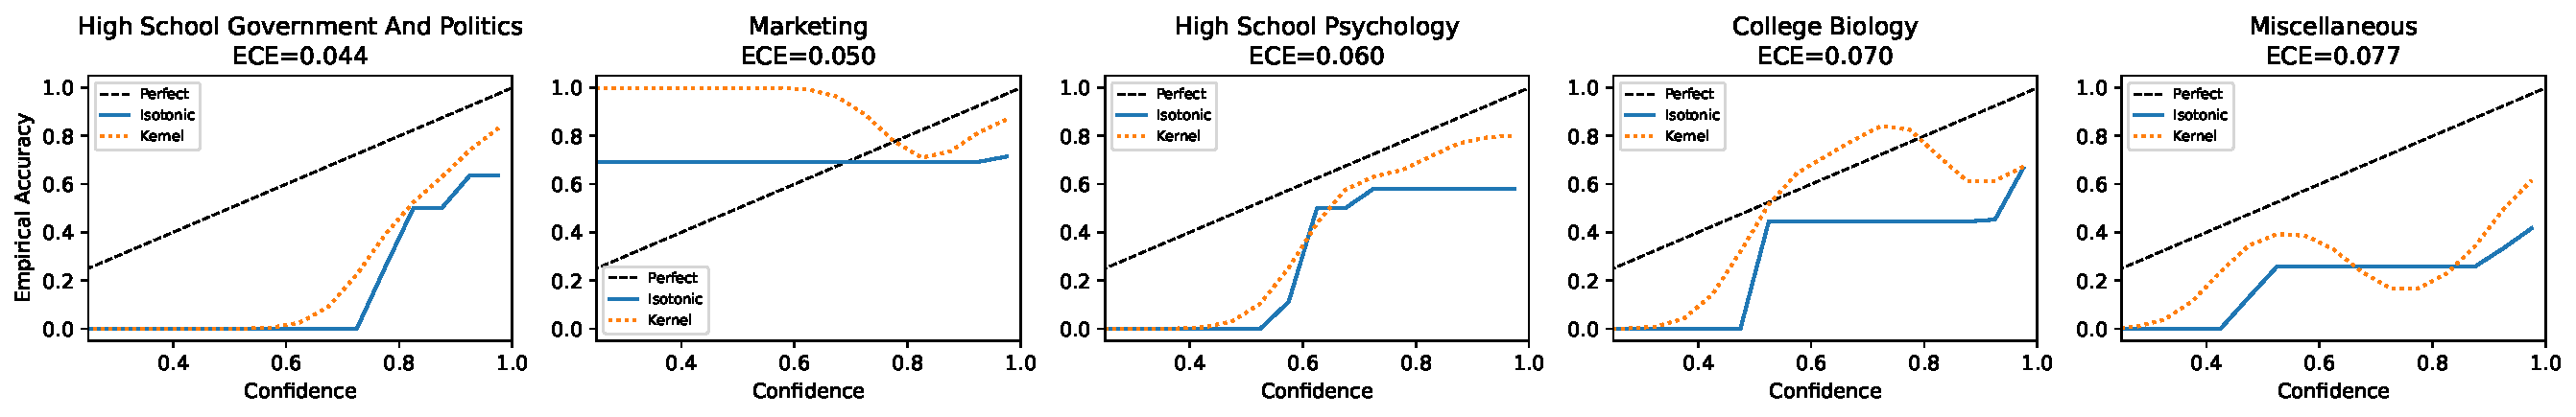
\includegraphics[width=0.95\linewidth]{bottom5_calibrated_gpt4o.pdf}
      \end{center}
      {\small GPT-4o-mini's own five most miscalibrated (top) and five
      best-calibrated (bottom) subjects by ECE --- the cross-model-robust
      worst/best list above differs slightly since it requires agreement
      across all seven models (see Cross-Model Stability). Solid: isotonic
      fit; dotted: kernel smoother; dashed: perfect calibration.}
    \end{block}

  \end{column}

  % ------------------------ Middle column -------------------------
  \begin{column}{0.34\linewidth}

    \begin{block}{Magnitude of Miscalibration}
      \begin{itemize}
        \item For each of the 57 subjects $s$, test whether its mean gap is
          zero:
      \end{itemize}
      \[
        H_0:\ \mathbb{E}\!\left[\mathrm{gap}_i \mid \text{subject } s\right] = 0
        \quad\text{vs.}\quad
        H_1:\ \mathbb{E}\!\left[\mathrm{gap}_i \mid \text{subject } s\right] \neq 0,
      \]
      \begin{itemize}
        \item One-sample $t$-tests, FDR-controlled at $\alpha=0.05$
          (Benjamini--Hochberg, 1995). Rejections are near-universal (five
          of seven models reject all 57) --- expected given the sample
          size, \emph{not informative} on its own.
      \end{itemize}

      \vspace{0.3em}
      \begin{center}
        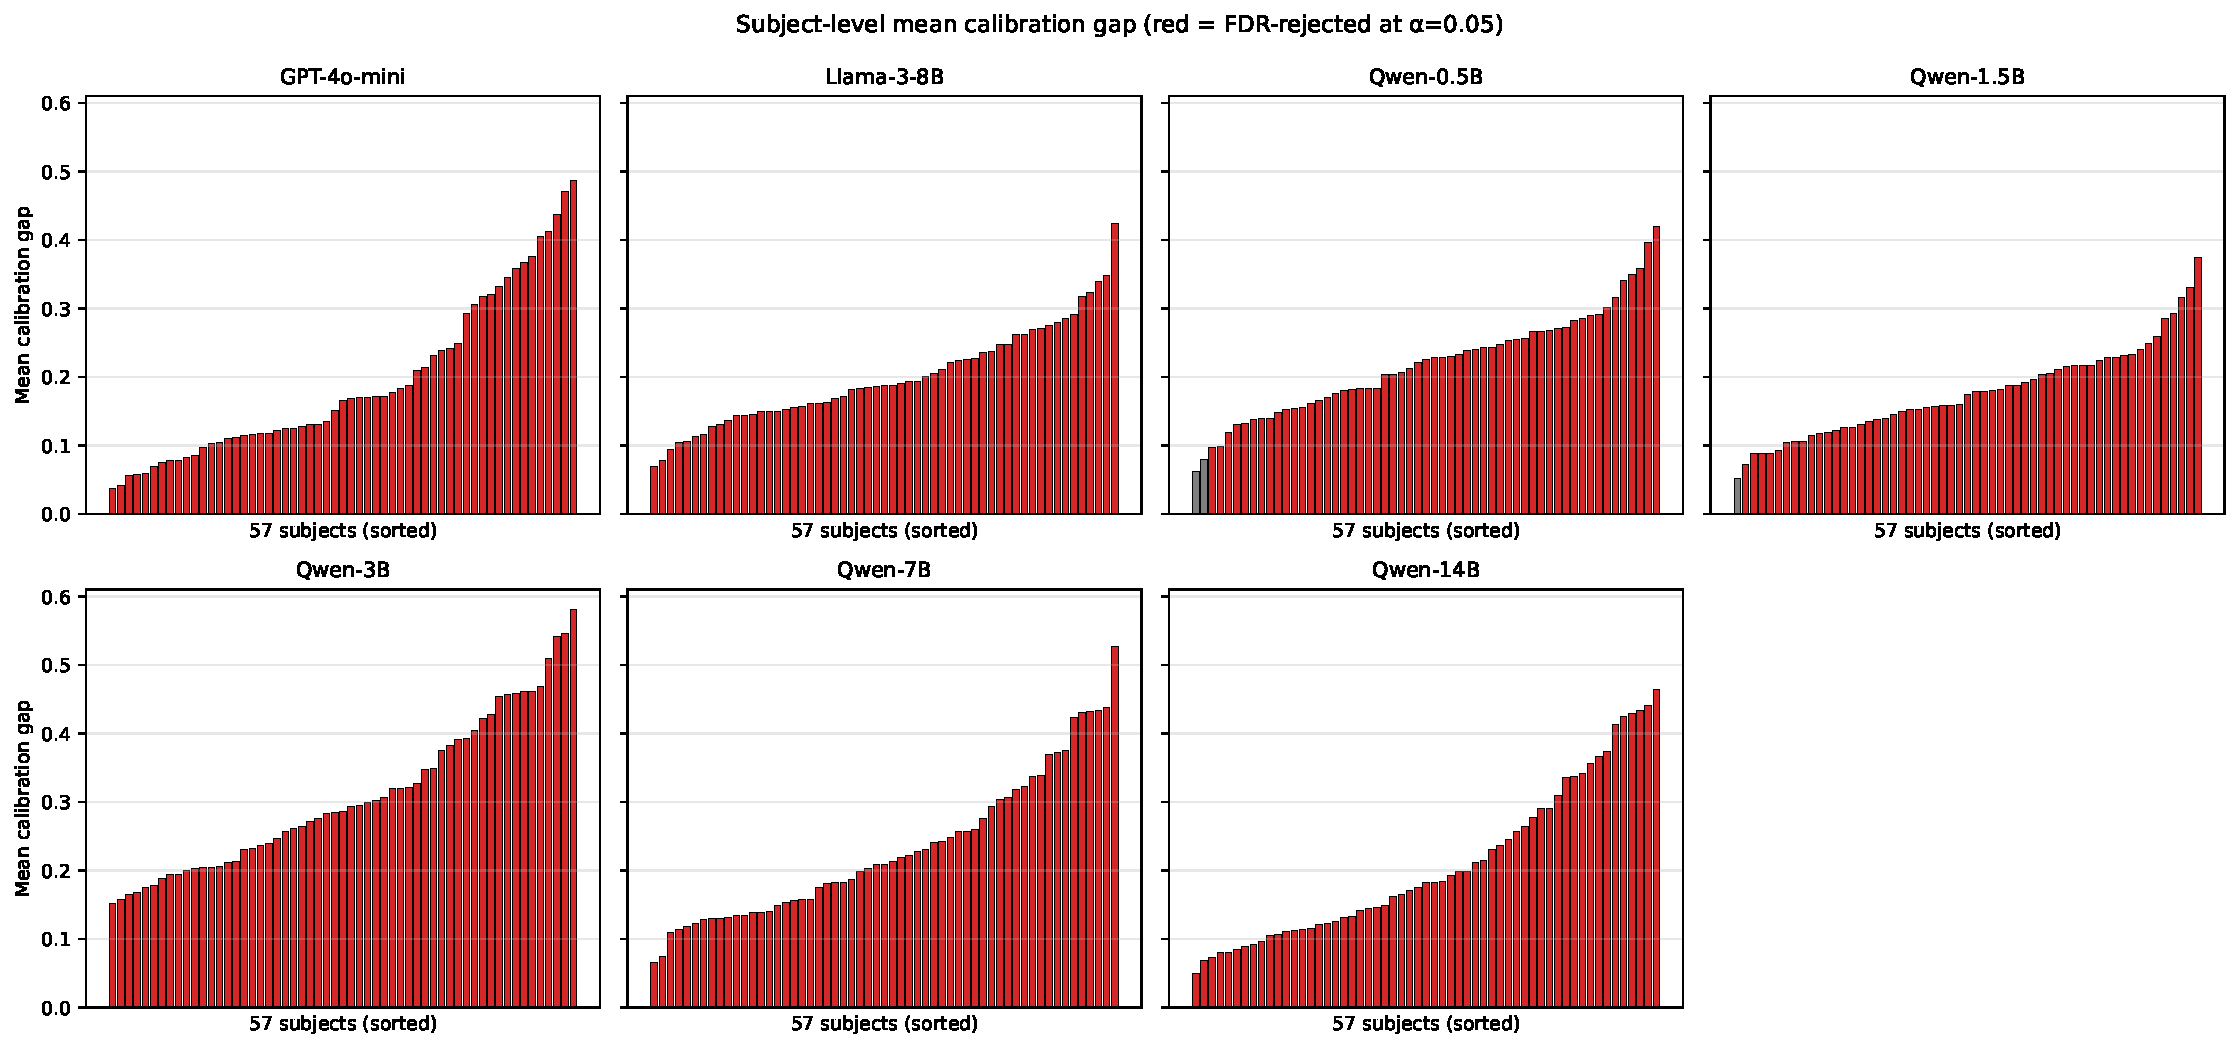
\includegraphics[width=0.56\linewidth]{subject_mean_gap_7m.pdf}
      \end{center}
      {\small Mean calibration gap per subject, sorted ascending, per
      model. Red bars: FDR-rejected at $\alpha=0.05$.}

      \vspace{0.2em}
      \begin{itemize}
        \item The real finding is the \emph{magnitude}: best- to
          worst-calibrated gap ranges span $3.8$--$13.0\times$ across the
          six larger models, and the \emph{same} subjects sit at each
          extreme, every time (robust to bin count and choice of scoring
          rule).
      \end{itemize}
    \end{block}

    \begin{block}{Stable Across Models and Families}
      \begin{itemize}
        \item All 15 pairwise Spearman correlations among the six larger
          models fall in $[0.80, 0.94]$.
        \item Cross-family GPT-4o-mini vs.\ Qwen-7B/14B ($0.92/0.91$) is as
          strong as the best within-family pair (Qwen-7B vs.\ 14B, $0.94$)
          --- the same subjects are hard \emph{regardless of architecture
          or scale}.
        \vspace{0.3em}
        \item Qwen-0.5B is a conspicuous exception ($\rho \in [0.13, 0.20]$,
          CIs include zero): it predicts D 59\% of the time vs.\ A 5.6\%, so
          its confidence tracks answer position, not item difficulty --- its
          subject ranking isn't a meaningful calibration signal below
          $\sim$1B parameters.
      \end{itemize}

      \vspace{0.4em}
      \begin{center}
        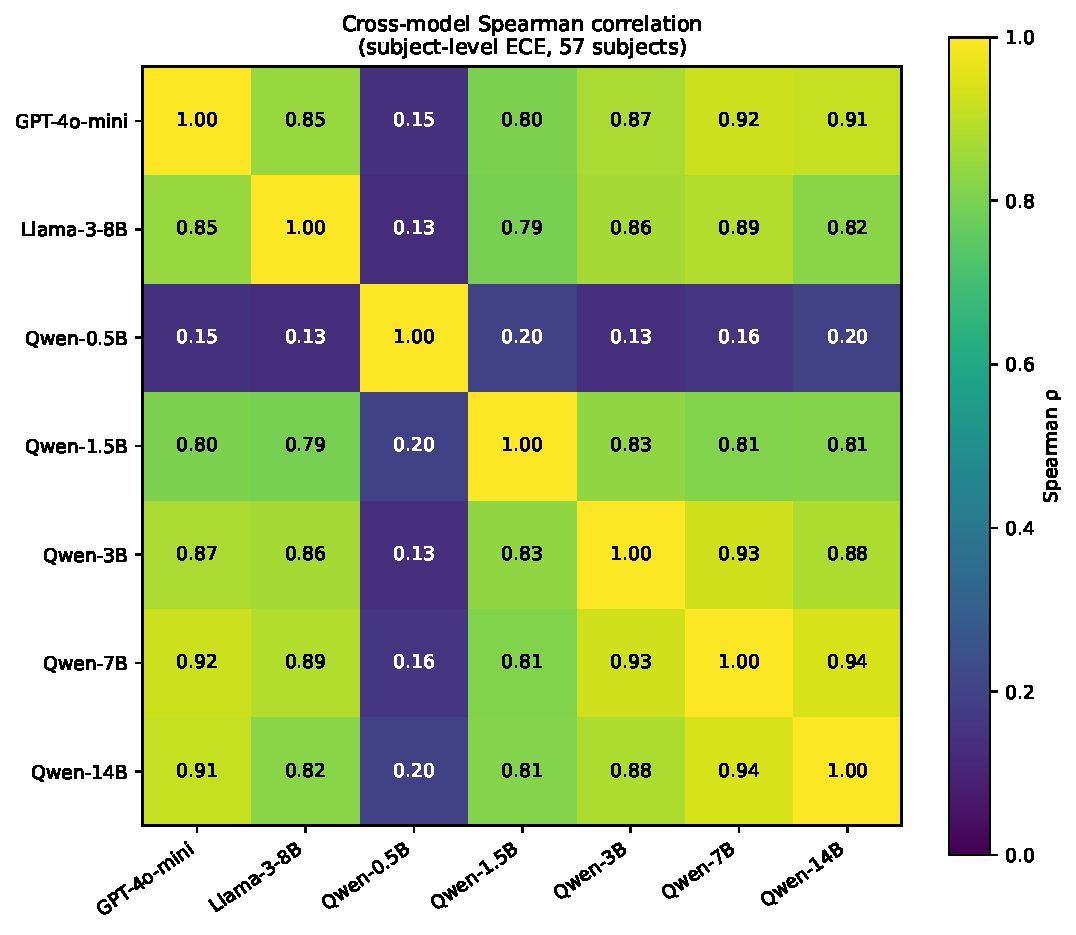
\includegraphics[width=0.42\linewidth]{cross_model_heatmap_7m.pdf}
      \end{center}
      {\small Spearman rank correlation of subject-level ECE across the seven
      models (57 common subjects).}
    \end{block}

    \begin{block}{What Predicts the Gap}
      \begin{itemize}
        \item Word count positively predicts overconfidence for
          GPT-4o-mini and the larger Qwens.
        \item Negation and option length: mostly inert.
        \vspace{0.3em}
        \item Most informative pattern: the \textbf{entropy} coefficient
          (next panel).
      \end{itemize}

      \vspace{0.4em}
      \begin{center}
        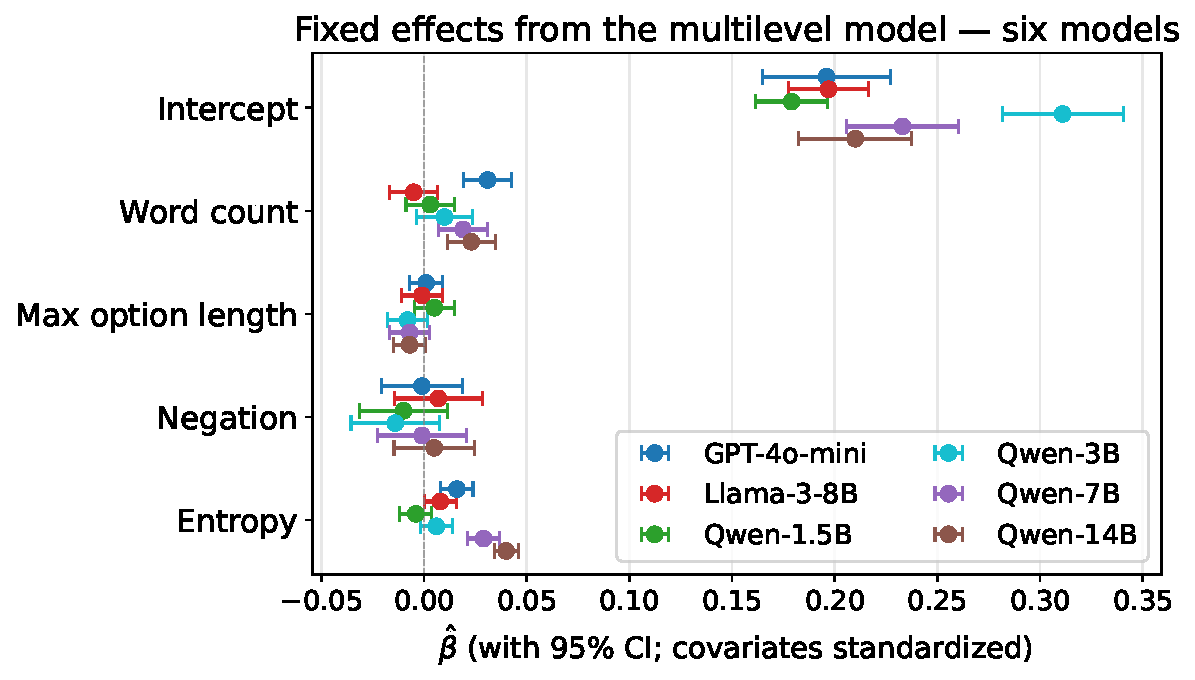
\includegraphics[width=0.68\linewidth]{coef_plot_7m.pdf}
      \end{center}
      {\small Fixed-effect estimates ($\pm$95\% CI) on the standardized
      calibration-gap scale, six models (Qwen-0.5B excluded --- positional
      bias, see Cross-Model Stability). The entropy coefficient shows a
      clear sign progression across the Qwen scaling sweep.}
    \end{block}

  \end{column}

  % ------------------------- Right column -------------------------
  \begin{column}{0.33\linewidth}

    \begin{block}{The Gap Grows With Scale}
      \begin{itemize}
        \item \textbf{Naive prediction:} higher entropy (harder item)
          should mechanically lower confidence, shrinking the gap.
        \vspace{0.3em}
        \item \textbf{What happens instead:} confidence \emph{does} drop as
          entropy rises, as predicted --- but accuracy drops faster still,
          so the gap widens on the hardest items.
        \vspace{0.3em}
        \item \textbf{Gets worse with scale:} the entropy coefficient flips
          sign across the Qwen sweep (1.5B $\to$ 14B, right).
      \end{itemize}

      \vspace{0.4em}
      \begin{center}
        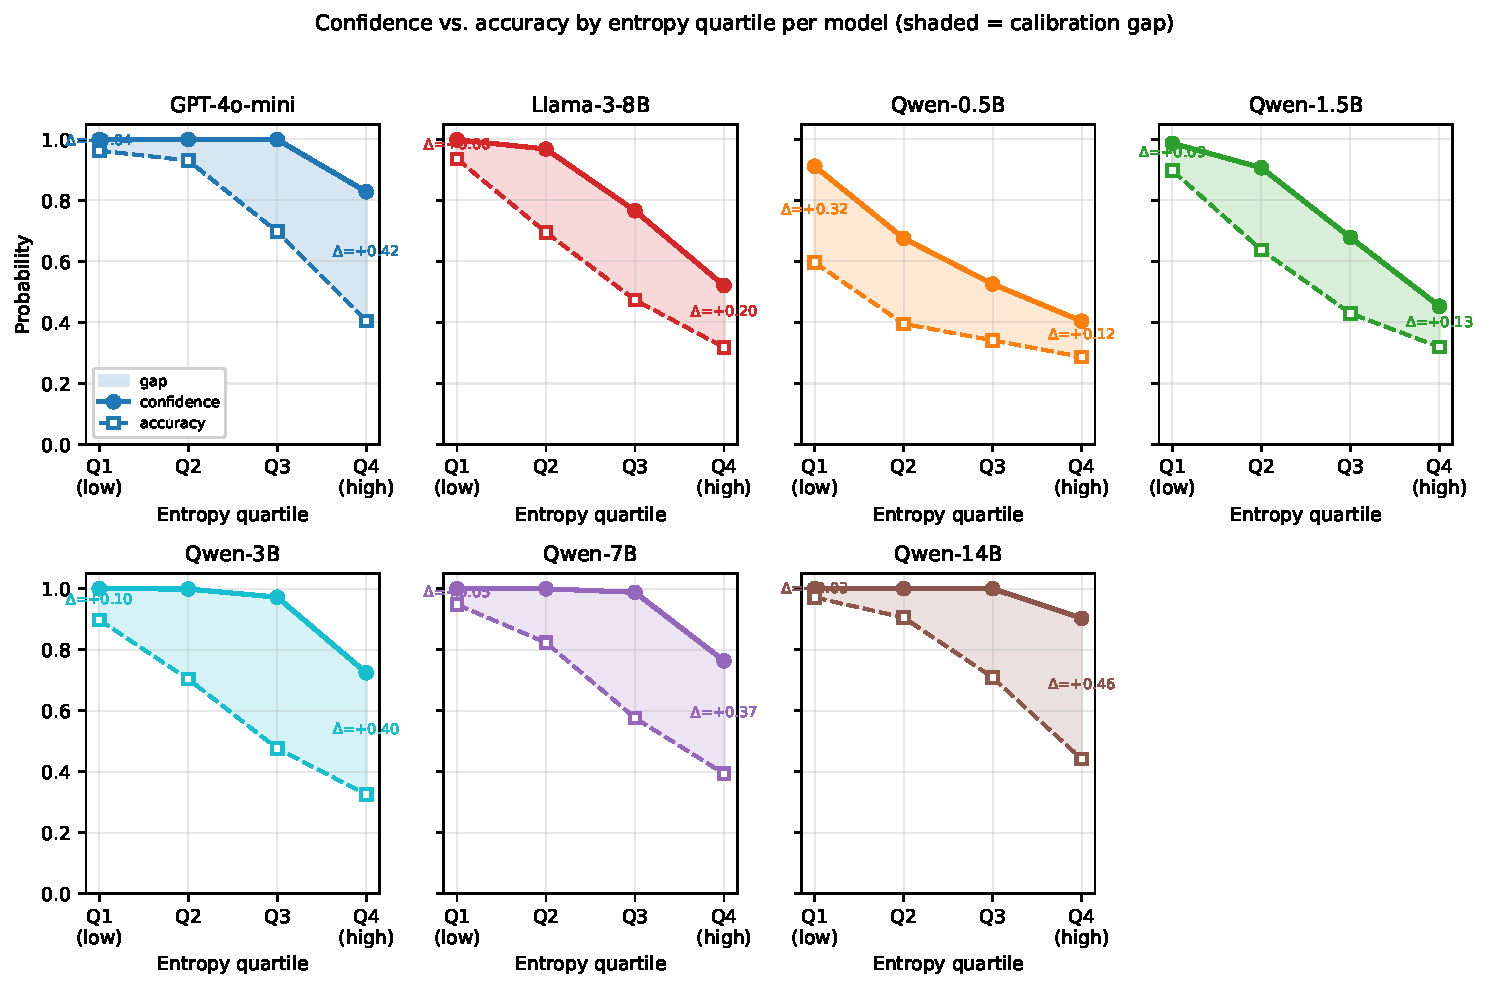
\includegraphics[width=0.55\linewidth]{entropy_mechanism_7m.pdf}\hfill
        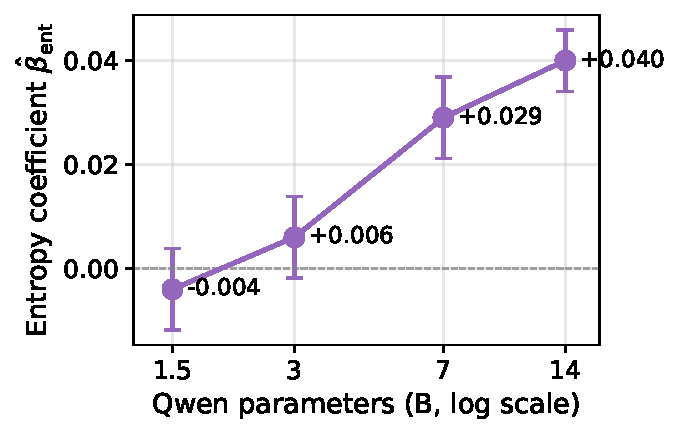
\includegraphics[width=0.42\linewidth]{entropy_scale_coef.pdf}
      \end{center}
      {\small Left: confidence (solid) and accuracy (dashed) by entropy
      quartile, shaded = calibration gap. Right: entropy coefficient
      $\hat\beta_\text{ent}$ across the Qwen scaling sweep ($\pm$95\% CI).}
    \end{block}

    \begin{block}{Robustness Checks}
      \begin{itemize}
        \item \textbf{ECE ranking:} $\rho \geq 0.97$ across bin counts
          $10$--$30$ vs.\ the 20-bin baseline, and $\rho \geq 0.79$ against
          the Negative Log Calibration Score, a bin-free proper scoring
          rule.
        \vspace{0.3em}
        \item \textbf{Variance decomposition:} two-level and three-level ICC
          estimates match exactly --- domain variance really is zero.
        \vspace{0.3em}
        \item \textbf{FDR threshold:} rejections hold at $\alpha=0.01$ too:
          55--57/57 for the four largest models, 46--55/57 for the smaller
          Qwens.
      \end{itemize}
    \end{block}

    \begin{block}{Takeaways}
      \begin{itemize}
        \item \textbf{The unit of analysis is the subject, not the model.}
          A single aggregate scalar hides a $3.8$--$13.0\times$ range in
          miscalibration magnitude --- a single global fix (e.g.\
          temperature scaling) can't work either: one scalar $T$ tuned for
          the worst subjects (\texttt{professional\_law}, \texttt{virology},
          gap up to $0.487$) would badly overcorrect well-calibrated
          subjects like \texttt{marketing} (gap $0.037$).
        \vspace{0.3em}
        \item \textbf{Miscalibration is task-driven.} Subject rankings are
          stable across three families and six scales
          ($\rho \in [0.80,0.94]$) --- model-level retraining is unlikely to
          resolve it; the fix has to live at the subject level.
        \vspace{0.3em}
        \item \textbf{Practical upshot:} the recurring worst-calibrated
          subjects double as a portable pre-deployment checklist --- flag
          likely miscalibration on a \emph{new} model without re-running the
          full 57-subject audit.
        \vspace{0.3em}
        \item \textbf{Open question:} \emph{why} these subjects are hardest
          (abstractness, training-data rarity, or something else) remains
          unresolved.
        \vspace{0.3em}
        \item \textbf{Caveats:} confidence is a single top-token logprob and
          may understate internal uncertainty post-RLHF; results are specific
          to MMLU's four-choice format; the Qwen scaling comparison spans
          only four checkpoints.
        \vspace{0.3em}
        \item \textbf{The audit generalizes:} the same multilevel-model +
          FDR pipeline applies to any benchmark with hierarchical structure
          --- next steps include a fourth model family at matched scale and
          replication on MMLU-Pro.
      \end{itemize}
    \end{block}

    \begin{block}{References}
      \begin{itemize}
        \item Benjamini \& Hochberg (1995). Controlling the false discovery
          rate. \emph{JRSS-B} 57(1).
        \vspace{0.8em}
        \item Guo et al.\ (2017). On calibration of modern neural networks.
          \emph{ICML}.
        \vspace{0.8em}
        \item Hendrycks et al.\ (2021). Measuring massive multitask language
          understanding. \emph{ICLR}.
        \vspace{0.8em}
        \item Kadavath et al.\ (2022). Language models (mostly) know what
          they know. arXiv:2207.05221.
        \vspace{0.8em}
        \item Nakkiran et al.\ (2025). Trained on tokens, calibrated on
          concepts. arXiv:2511.04869.
        \vspace{0.8em}
        \item Xiong et al.\ (2024). Can LLMs express their uncertainty?
          \emph{ICLR}.
      \end{itemize}
    \end{block}
  \end{column}

\end{columns}

\end{frame}
\end{document}
